\documentclass[11pt]{article}

% acl.sty modes:
%   preprint - author names shown, page numbers, no line numbers  (current)
%   review   - ANONYMISED ("Anonymous ACL submission"), line numbers, page
%              numbers. Use this only when submitting somewhere double-blind.
%              Line numbers make it much easier to give feedback by reference,
%              so switch to it for a commenting round if that helps.
%   final    - author names shown, no line numbers, no page numbers. Camera-ready.
\usepackage[preprint]{acl}
\usepackage{times}
\usepackage{latexsym}
\usepackage[T1]{fontenc}
\usepackage[utf8]{inputenc}
\usepackage{microtype}
\usepackage{inconsolata}
\usepackage{graphicx}
\usepackage{booktabs}
\usepackage{makecell}
\usepackage{enumitem}
\definecolor{hit}{HTML}{1B7F4B}
% Visible collaboration macros. Keep this file in review builds.
\usepackage{xcolor}
\usepackage[normalem]{ulem}

\newcommand{\draftcomment}[3]{{\textcolor{#3}{[\textsc{#1}: #2]}}}
\newcommand{\resolved}[1]{}
\newcommand{\opennote}[1]{\draftcomment{open}{#1}{teal}}
\newcommand{\placeholder}[1]{{\textcolor{red}{\textbf{[#1]}}}}

% Nimrod Segev
\newcommand{\nimrod}[1]{\draftcomment{nimrod}{#1}{blue}}
\newcommand{\nimroda}[1]{\textcolor{blue}{[#1]}}
\newcommand{\nimrods}[1]{\nimrod{\sout{#1}}}
\newcommand{\nimrodr}[2]{\nimrods{#1}\nimroda{#2}}

% Yuval Reif
\newcommand{\yuval}[1]{\draftcomment{yuval}{#1}{violet}}
\newcommand{\yuvala}[1]{\textcolor{violet}{[#1]}}
\newcommand{\yuvals}[1]{\yuval{\sout{#1}}}
\newcommand{\yuvalr}[2]{\yuvals{#1}\yuvala{#2}}

% Roy Schwartz
\newcommand{\roy}[1]{\draftcomment{roy}{#1}{teal}}
\newcommand{\roya}[1]{\textcolor{teal}{[#1]}}
\newcommand{\roys}[1]{\roy{\sout{#1}}}
\newcommand{\royr}[2]{\roys{#1}\roya{#2}}

% Agent-proposed changes remain visible until an author accepts them.
\newcommand{\unapprovedcomment}[1]{\draftcomment{agent}{#1}{orange}}
\newcommand{\ma}[1]{\textcolor{orange}{[#1]}}
\newcommand{\ms}[1]{\unapprovedcomment{\sout{#1}}}
\newcommand{\mr}[2]{\ms{#1}\ma{#2}}

% For a clean local reading copy, uncomment only these display overrides.
% Do not commit a submission build with unresolved edits or comments.
% \renewcommand{\draftcomment}[3]{}
% \renewcommand{\ma}[1]{#1}
% \renewcommand{\ms}[1]{}


\title{Do Language Models Recognize a Phrase Before Reading It?}
% Names and shared affiliation only; no contact addresses, by the authors'
% choice. acl.sty imposes no author format, so add addresses back here if a
% venue wants them.
\author{
  Nimrod Segev \quad Yuval Reif \quad Roy Schwartz \\[2pt]
  School of Computer Science and Engineering \\
  The Hebrew University of Jerusalem
}

\begin{document}
\maketitle
\begin{abstract}
Language models emit one token per forward pass, yet some continuations are
effectively fixed several tokens in advance. We ask whether a model's hidden
state, partway through a familiar multi-word expression, already carries enough
information to recover the rest of it. Interrupting OLMo-2-7B at a controlled
\emph{lookahead distance} $i$ across $1{,}164$ idioms, landmark names and film
titles, in isolation and in $9{,}955$ naturally occurring contexts, we find that
it often does: the model produces
the final three tokens of a phrase in $64.8\%$ of in-context instances and the
final five in $53.6\%$, against $31.2\%$ and $17.6\%$ for the same phrases
presented alone. Which phrase it is matters far more than which sentence it appears in: given
several natural contexts, a phrase tends either to be recovered in almost all of
them or in almost none. The signal is legible from the representation itself,
and a small probe reading a single hidden state predicts whether the model will
complete the phrase at $87.6\%$ precision, before any of it is generated.
Comparing the two readouts on identical instances, Patchscopes systematically
undercounts what the model does: generation recovers continuations it misses
about three times as often as the reverse, and much of that gap turns out to be
the number of layers we chose to sweep rather than anything about the model.
Trained on the two readouts' labels, the same probe places the signal in
different parts of the network. Anticipation is there to be measured; how much
one finds, and where, depends on the instrument.
\end{abstract}

\section{Introduction}
\label{sec:intro}

A decoder-only language model emits one token per forward pass, and pays the
full depth of the network for each one. This is not obviously necessary. Some
continuations are all but fixed by the time the model has read a few tokens:
after \textit{the Empire}, in a sentence about New York, very little other than
\textit{State Building} can follow. If the model's hidden state at
\textit{Empire} already encodes \textit{State Building}, then the two forward
passes that produce those tokens are, in an information-theoretic sense,
re-deriving something the model had already computed.

Recent interpretability work has shown that language models do build
representations of units larger than a single token. \citet{kaplan-etal-2025-tokens}
demonstrate an \emph{intrinsic detokenization} process: when a word is split
into several subword tokens, information from the earlier pieces is aggregated
into the last one, and the resulting state behaves like a representation of the
whole word, even for words the tokenizer never emits as a unit. That result,
however, concerns a unit the model has \emph{already finished reading}. It
establishes that the model consolidates evidence backwards, not that it
anticipates forwards. The question we ask here is the forward one, and it is
the one with consequences for how models are run:

\begin{quote}
Given a partial phrase, does the model's internal representation already encode
the rest, before it has read or generated any of it?
\end{quote}

We study this for \emph{fixed multi-word expressions} --- idioms, landmark
names, and film titles --- because for these the continuation is well defined,
and because their frequency in pretraining data makes them the most favourable
case. If anticipation does not happen here, it is unlikely to happen anywhere.
We index the question by \emph{lookahead distance} $i$: the number of phrase
tokens still unread at the point where we interrupt the model. At $i=4$ in
\textit{The Lord of the Rings}, the model has read only \textit{The}, and we ask
whether \textit{Lord of the Rings} is recoverable from its state.

Recoverable by what means, however, turns out to matter as much as the answer.
We use two readouts on the same interrupted states. The first is
Patchscopes \citep{ghandeharioun-etal-2024-patchscopes}: we lift the hidden
state at the cut position and inject it into an unrelated prompt, and ask
whether the model verbalises the remaining tokens. The second simply lets the
model continue generating from the true prefix it has actually seen. The first
asks what a vector contains; the second asks what the model does. Prior work
treats a successful Patchscopes readout as evidence that the model ``knows''
something, and we wanted to know how far that licence extends.

Our findings are as follows. Phrase-level anticipation is real and substantial:
in natural context, OLMo-2-7B produces the final two tokens of a familiar phrase
in $84.0\%$ of instances, and the final five in $53.6\%$, against $59.2\%$ and
$17.6\%$ for the same phrases in isolation (\S\ref{sec:lookahead}). It is a
stable property of the phrase rather than of the occasion: per-phrase success at
$i=3$ is far more bimodal than independent per-context variation would produce,
with $31.5\%$ of phrases succeeding in at least $90\%$ of their contexts against
a binomial expectation of $10.1\%$ (\S\ref{sec:stability}). And the signal is
decodable: a small
classifier reading the raw hidden state predicts whether the model will in fact
complete the phrase at $76.8\%$ balanced accuracy and $87.6\%$ precision
(\S\ref{sec:probe}).

The two readouts, however, do not measure the same thing. Run on identical
instances, they agree on only $81.1\%$ of them, and their disagreements run in
both directions --- $1{,}924$ instances recovered only by Patchscopes against
$2{,}751$ recovered only by generation (\S\ref{sec:disagreement}). They order
the three phrase categories differently, and the two probes trained on their
respective labels place the ``best'' layer in different parts of the network.
We take this as a caution rather than a refutation: Patchscopes remains
informative about representational content, but a claim of the form \emph{the
model knows $X$ at layer $\ell$} is not readout-independent, and should say
which instrument produced it.

Concretely, we contribute:

\begin{enumerate}[nosep,leftmargin=*]
\item A lookahead-distance protocol for measuring phrase anticipation, applied
      to $1{,}164$ fixed expressions both in isolation and in $9{,}955$
      naturally occurring FineWeb-Edu contexts, with two independent readouts
      run on identical instances (\S\ref{sec:method}).
\item Evidence that anticipation of familiar phrases occurs several tokens
      ahead, is greatly strengthened by natural context, and is a stable
      property of the phrase (\S\ref{sec:lookahead}--\S\ref{sec:stability}).
\item A direct comparison showing that the two readouts disagree substantially
      and asymmetrically, and that conclusions about category difficulty and
      layer localisation depend on which one is used
      (\S\ref{sec:disagreement}).
\item A hidden-state probe that predicts real completion success well above
      chance from the first transformer layer onward, together with an
      adjudication of its apparent errors showing that roughly four in five are
      valid alternate phrasings rather than failures (\S\ref{sec:probe}).
\end{enumerate}

\section{Related Work}
\label{sec:related}

\paragraph{Representations of units larger than a token.}
The closest earlier work is \citet{kaplan-etal-2025-tokens}, who show
that when a word is split into several subword tokens, early attention
aggregates the pieces into the final subtoken and feed-forward layers then write
a whole-word representation into that position. They read these states out with
Patchscopes and find that the model can regenerate words for which no single
vocabulary token exists, which they interpret as a latent lexicon broader than
the tokenizer's vocabulary. Their unit is a word the model has finished reading; ours is a phrase it has
not. The two share a method but not a claim: pulling together evidence already
seen is a weaker thing than anticipating evidence not yet seen.
\citet{reif-etal-2026-vocab} build on the same picture to reshape model
vocabularies, and \citet{artzy-schwartz-2024-attend} add evidence that attention
gathers information early and later layers work on the result.

\paragraph{Idioms and memorised sequences.}
\citet{haviv-etal-2023-understanding} study how transformers recall memorised
idiom completions, and find the process to be two-stage: early layers promote
the memorised token to the top of the output distribution, and upper layers
raise the model's confidence in it. They study how a single target token is recalled; we measure how far ahead
recall reaches and how it varies across phrases and sentences. Our idiom set is drawn from
MAGPIE \citep{haagsma-etal-2020-magpie} and
LIdioms \citep{moussallem-etal-2018-lidioms}.

\paragraph{Anticipating future tokens from one hidden state.}
Our question was posed, in a more general form, by Future
Lens \citep{pal-etal-2023-future}: given the hidden state of a single token at
position $t$, can the tokens at positions $\geq t+2$ be recovered? They answer
it with linear approximation and with causal intervention (transplanting the
state into a different context and reading what the model then produces), and
report better than $48\%$ accuracy at some layers of GPT-J-6B. That transplant
is the technique Patchscopes later generalised, and our Patchscopes readout is a
direct descendant of it.

We differ in what is anticipated and in what it is checked against. Future Lens
scores the recovered tokens against whatever the model would have written next;
we score them against the phrase, which is fixed in advance and does not move
with the model. That lets us repeat a phrase across many sentences
(\S\ref{sec:stability}) and set the transplant against the model's own writing
on matched instances (\S\ref{sec:disagreement}). Future Lens compares two
\emph{decoding} methods against the model's output; we compare a decoding
method against the model's behaviour, and find that they disagree in ways that
change conclusions.

\paragraph{Reading hidden states.}
The logit lens \citep{nostalgebraist-2020-logitlens} projects an intermediate
state through the unembedding to ask what token it would predict.
Patchscopes \citep{ghandeharioun-etal-2024-patchscopes} generalises both it and
the Future Lens intervention by injecting the state into an arbitrary prompt and
letting the model write it out, which lifts the restriction that the answer be
a single vocabulary item and so allows multi-token readouts. All three act on a representation at inference time, and all raise the same
question: is what comes out what the model would otherwise have used? We test
that directly in \S\ref{sec:disagreement}.

\paragraph{Probing internal states for future correctness.}
\citet{orgad-etal-2025-llms} show that hidden states encode more about the
truthfulness of a forthcoming answer than the output distribution reveals, that
the signal concentrates in particular tokens, and that probes trained on it
generalise poorly across datasets. Our probe is the same kind of thing pointed at a different question, not whether
an answer will be true but whether a phrase will be finished, and it behaves
similarly, including the limited transfer across categories in
Appendix~\ref{app:details}. In a similar spirit,
\citet{gekhman-etal-2024-fine} treat a model's pre-existing knowledge of an item
as a measurable quantity predicting downstream behaviour.

\paragraph{Exploiting anticipation for efficiency.}
If a model's state already determines several upcoming tokens, that redundancy
can be spent. Speculative decoding \citep{leviathan-etal-2023-fast} drafts
several tokens with a cheaper process and verifies them with the target model;
multi-token prediction heads \citep{gloeckle-etal-2024-better} train the model
to emit several tokens at once; and LayerSkip
\citep{elhoushi-etal-2024-layerskip} exits early and self-speculates.
\citet{aynetdinov-akbik-2025-babies} show that a multi-token prediction
objective helps even 130M-parameter models under severe data constraints,
suggesting the capacity to train for lookahead is not confined to large models.

Closest to the use our probe suggests is CLP \citep{xie-zhou-2026-clp}, which
trains one small linear layer on the hidden state to set how many drafted tokens
to accept at each step, reporting $1.14\times$--$1.29\times$ on Qwen2.5 without
measurable quality loss: the same kind of read as our probe, used to make a
decoding decision rather than to answer a question. All of these methods assume
useful anticipation exists. We measure it directly, for one well-defined class
of continuations, and say when it is reliable. We implement no decoding
method here and report no speed-ups of our own.

\section{Measuring Phrase Anticipation}
\label{sec:method}

\begin{figure*}[t]
\centering
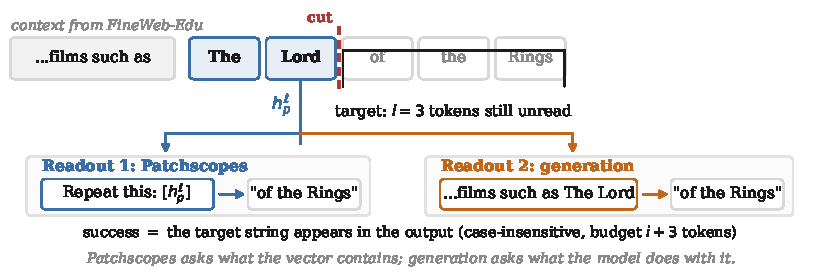
\includegraphics[width=\textwidth]{figures/protocol}
\caption{The protocol. We interrupt the model inside a known phrase, leaving $i$
tokens unread, and ask whether those tokens are recoverable from that point by
two different means: injecting the hidden state into an unrelated prompt
(Patchscopes), or letting the model continue from the prefix it has actually
seen (generation). Both are scored identically. In both, only the first token is
produced from the state shown; decoding then continues autoregressively, so a
multi-token recovery does not imply that every token was separately encoded in
$h^{\ell}_p$.}
\label{fig:protocol}
\end{figure*}

Figure~\ref{fig:protocol} summarises the protocol.

\subsection{Lookahead distance}

Let a phrase tokenize as $t_1 \ldots t_n$. We interrupt the model at position
$p$ and define the \emph{lookahead distance} $i = n - p$ as the number of phrase
tokens that remain unread. The target is the decoded string of those $i$ tokens.
A single phrase therefore yields several trials, one per position, and $i$ is
the difficulty axis throughout: larger $i$ means the model must account for more
unseen material.

Every phrase is processed with its full left context (a BOS token, then,
where applicable, the natural text preceding the phrase), so the state at
position $p$ is the state the model would actually have at that point. We analyse
$i \geq 2$ throughout; $i=1$ reduces to ordinary next-token prediction and is
not of interest here.

\subsection{Two readouts}
\label{sec:readouts}

We ask whether the remaining tokens are recoverable from the model at position
$p$ in two ways. Both take the same input and differ only in what is done with
it.

\paragraph{Patchscopes readout.}
Following \citet{ghandeharioun-etal-2024-patchscopes}, and ultimately the causal
intervention of \citet{pal-etal-2023-future}, we take the hidden state
$h^{\ell}_p$ at layer $\ell$ and position $p$, and substitute it for the token
embedding of \texttt{X} in the prompt \texttt{"Repeat this: X"}. We then decode
greedily for $i+3$ tokens. The readout succeeds at layer $\ell$ if the target
string occurs in the output, case-insensitively. Unless stated otherwise we
report the union over layers: the readout succeeds if \emph{any} probed layer
succeeds. This is a deliberately generous criterion, and \S\ref{sec:disagreement}
shows that how many layers enter the union materially changes the result.

\paragraph{Generation readout.}
We take the same prefix, context plus the first $p$ phrase tokens, and let
the model generate greedily for $i+3$ tokens, with no intervention of any kind.
The readout succeeds under the same string-containment criterion.

Neither readout is ground truth for the other, and they are not two decoders of
the same object. Patchscopes intervenes on a single hidden state and asks what
that vector can be made to express; generation runs the full model on the
matched prefix and asks what it does. The comparison is therefore between
representational extractability and behaviour, and we treat them as two
instruments rather than two views (\S\ref{sec:disagreement}).

One consequence is worth stating before any results. Both readouts decode
autoregressively, so a recovered target of several tokens does not show that
each of those tokens is separately encoded in the cut-position state: after the
first generated token, the rest may follow from what has already been emitted.
What a success shows is that the state carries enough information to elicit the
continuation under that readout. We use \emph{recognition} and
\emph{anticipation} in that operational sense throughout: a phrase is
recognized at distance $i$ when a named readout recovers its remaining $i$
tokens under the matching criterion below.

\subsection{Success criterion}
\label{sec:criterion}

A trial succeeds if the target string appears as a case-insensitive substring of
the generated continuation. The budget of $i+3$ tokens allows the model to
overshoot slightly (a trailing clause after the phrase does not cost it the
trial) while remaining tight enough that a success reflects the phrase
rather than a long ramble that happens to contain it.\footnote{An earlier
version of this work used a fixed five-token budget, which mechanically forced
zero successes at $i \geq 6$. The reported $i \geq 6$ rates here are the
corrected ones.}

The criterion is lenient in one direction and strict in the other. Lenient,
because it accepts any output containing the target without asking whether the
model produced it for the right reason; strict, because it demands the exact
wording: \textit{he who laughs last laughs \underline{best}} scores as a
failure against \textit{laughs loudest}, though it is the more common form.
\S\ref{sec:falsepos} quantifies how often that strictness misclassifies a
correct completion.

\section{Experimental Setup}
\label{sec:setup}

\begin{table}[t]
\centering\small
\begin{tabular}{lrrrl}
\toprule
 & \multicolumn{1}{c}{\textbf{Phrases}} & \multicolumn{1}{c}{\textbf{w/ ctx.}} & \multicolumn{1}{c}{\textbf{Inst.}} & \textbf{Example} \\
\midrule
Landmarks & 127 & 125 & 1,217 & \textit{the Great Wall of China} \\
Idioms & 852 & 802 & 7,230 & \textit{the grass is always greener\ldots} \\
Film titles & 185 & 169 & 1,508 & \textit{Harry Potter and the Goblet of Fire} \\
\midrule
Total & 1,164 & 1,096 & 9,955 & \\
\bottomrule
\end{tabular}
\caption{The phrase set. \textbf{Phrases} counts expressions long enough to
admit at least one lookahead position; \textbf{w/ ctx.} counts those for which
at least one natural occurrence was found in FineWeb-Edu; \textbf{Inst.} counts
(phrase, context) pairs, of which 925 phrases
contributed the full ten.}
\label{tab:dataset}
\end{table}


\subsection{Phrases}

We assemble $1{,}164$ fixed multi-word expressions of three kinds
(Table~\ref{tab:dataset}). \textbf{Idioms} ($852$) come from
MAGPIE \citep{haagsma-etal-2020-magpie} and
LIdioms \citep{moussallem-etal-2018-lidioms} together with two smaller
lists distributed with the same release.\footnote{\nimrod{The release also
labels $81$ items \texttt{EPIC} and $95$ across two \texttt{ep\_*} splits; we
should identify and cite their source before submission.}} \textbf{Landmarks}
($127$) are drawn from a curated list of well-known buildings and sites, and
\textbf{film titles} ($185$) are the multi-word entries of the IMDb Top 250.

The three kinds are chosen to vary the reason a continuation is predictable.
An idiom is fixed by convention, a landmark name by reference, and a film title
by citation --- but all three should be frequent in pretraining text, which is
what makes them a favourable test case. Phrases too short to admit a lookahead
position of at least $2$ are excluded.

\subsection{Natural contexts}

Fixed expressions in isolation are an artificial stimulus: the model sees a
bare phrase with no indication that a phrase is what it is looking at. We
therefore also collect natural occurrences. Streaming
FineWeb-Edu \citep{penedo-etal-2024-fineweb}, we search for surface occurrences
of each phrase and keep up to ten per phrase, each with up to $150$ tokens of
preceding text. For phrases that are predominantly capitalised --- most
landmarks and titles --- we require the occurrence to preserve at least $70\%$
of the original capitalisation, which prevents a sentence about sunrise from
being collected as an instance of the film \textit{Before Sunrise}.

This yields $9{,}955$ (phrase, context) instances covering $1{,}096$ of the
$1{,}164$ phrases, of which $925$ reach the full ten slots. Because the
collector resumed from an earlier five-context run and re-added the contexts it
already held rather than topping up with new ones, $44.8\%$ of these instances
are repeats: $734$ of the $925$ ten-slot phrases hold five distinct contexts
recorded twice, and there are $5{,}498$ distinct (phrase, context) pairs in
total. Decoding is greedy, so a repeat reproduces its original outcome exactly.
Aggregate rates over instances are therefore essentially unchanged --- $64.8\%$
versus $64.5\%$ at $i=3$ for the generation readout --- but the effective sample
size is roughly half the instance count, and any analysis that counts successes
\emph{per phrase} must deduplicate first. We report instance-level rates over
the full set for comparability with the per-layer and probing analyses, which
were run on it, and compute all per-phrase statistics (\S\ref{sec:stability})
over distinct contexts only. Each instance
contributes one trial per admissible lookahead distance, for a total of $27{,}098$
trials, $24{,}740$ of them at $i \in \{2,3,4,5\}$. Instance counts fall with $i$
because longer lookaheads require longer phrases: $9{,}148$ trials at $i=2$,
$8{,}529$ at $i=3$, $4{,}677$ at $i=4$ and $2{,}386$ at $i=5$.

Because idioms dominate the phrase set and tend to appear often in web text,
they also dominate the instance set ($20{,}371$ of $24{,}740$ pooled trials).
Aggregate rates over instances are therefore close to idiom rates, and we report
per-category results separately in \S\ref{sec:disagreement}.

\subsection{Models}

Our main model is OLMo-2-7B \citep{olmo-2025-olmo2} in \texttt{bfloat16}, a
$32$-layer decoder-only model chosen because its training data is public, which
makes the assumption that these phrases were seen in pretraining checkable in
principle. We replicate the central measurements on OLMo-3-7B and, for the
generation readout, on Qwen2.5-14B \citep{qwen-2024-qwen25}
(Appendix~\ref{app:details}).

For the Patchscopes readout we sweep all $32$ layers where the analysis permits
it. The probing experiments (\S\ref{sec:probe}) require storing hidden states
for every trial, so they use a fixed subset of eight layers
$\{5, 7, 10, 13, 15, 20, 25, 30\}$. \S\ref{sec:disagreement} shows that this
difference is not cosmetic, and we are explicit throughout about which layer set
a given number reflects.

\section{Results}
\label{sec:results}

\subsection{Phrases are recovered several tokens ahead}
\label{sec:lookahead}

\begin{table}[t]
\centering\small
\begin{tabular}{lrrrr}
\toprule
& \multicolumn{4}{c}{\textbf{Lookahead distance} $i$} \\
\cmidrule(lr){2-5}
\textbf{Readout / condition} & 2 & 3 & 4 & 5 \\
\midrule
\multicolumn{5}{l}{\textit{Phrase in isolation}} \\
\quad Patchscopes & 57.8 & 30.9 & 19.4 & 16.5 \\
\quad Generation & 59.2 & 31.2 & 20.6 & 17.6 \\
\midrule
\multicolumn{5}{l}{\textit{Phrase in natural context}} \\
\quad Patchscopes & 73.2 & 57.5 & 43.9 & 38.7 \\
\quad Generation & 84.0 & 64.8 & 55.6 & 53.6 \\
\midrule
\multicolumn{5}{l}{\textit{Robustness: wider Patchscopes layer sweep}} \\
\quad Patchscopes, all 32 layers & 79.6 & 64.1 & 51.6 & 46.4 \\
\bottomrule
\end{tabular}
\caption{Recovery rate (\%) of the final $i$ phrase tokens, OLMo-2-7B.
Isolation rows are computed over phrases
(1,112 at $i=2$); context rows over
(phrase, context) instances (9,148,
8,529,
4,677 and
2,386 at $i=2\ldots5$).
Patchscopes counts a success if \emph{any} probed layer recovers the
continuation, over the eight layers used throughout this paper
(\S\ref{sec:setup}); isolation rows sweep all 32. The final row re-runs the
in-context sweep over all 32 layers and is discussed in
\S\ref{sec:disagreement}.}
\label{tab:main}
\end{table}


\begin{figure}[t]
\centering
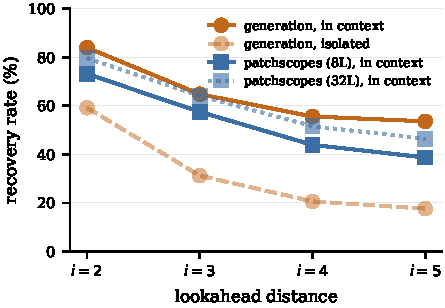
\includegraphics[width=\columnwidth]{figures/context_vs_isolation}
\caption{Recovery rate against lookahead distance. Natural context lifts the
generation readout by $25$--$36$ points over the same phrases in isolation. The
two Patchscopes curves are the same measurement under different layer budgets
and differ by $6$--$8$ points, which is most of the apparent gap to generation
(\S\ref{sec:disagreement}).}
\label{fig:context}
\end{figure}

Table~\ref{tab:main} gives the central measurement. In natural context,
OLMo-2-7B completes a familiar phrase two tokens early in $84.0\%$ of instances,
three tokens early in $64.8\%$, and five tokens early in $53.6\%$. Anticipation
of fixed expressions is therefore not a marginal effect at short range; it
persists at distances of several tokens, well past the horizon of ordinary
next-token prediction.

\paragraph{Isolation understates the effect.}
The same phrases presented alone, with no surrounding text, are recovered far
less often: $59.2\%$ at $i=2$ falling to $17.6\%$ at $i=5$ (Figure~\ref{fig:context}).
The gap widens with distance, from $24.8$ points at $i=2$ to $36.0$ points at
$i=5$, and the Patchscopes readout shows the same pattern. This is the expected
direction --- context supplies both topical evidence and the signal that a fixed
expression is under way --- but its size matters for interpreting prior
results. A bare phrase is a poor proxy for the condition
under which a model actually encounters these expressions, and measurements
taken in isolation should be read as a lower bound.

\paragraph{Successes persist beyond the range we analyse.}
We restrict the main analysis to $i \leq 5$ because instance counts fall
steeply beyond that. The effect does not stop there, however: in context,
generation recovers $48.9\%$ of the $1{,}123$ trials at $i=6$ and $41.7\%$ of
the $312$ at $i=8$. We do not draw conclusions from the sparse tail, but we note
it because an earlier version of this work reported zero successes at
$i \geq 6$; that was an artifact of a fixed generation budget
(\S\ref{sec:criterion}), not a property of the model.

\subsection{Anticipation is a property of the phrase}
\label{sec:stability}

\begin{figure}[t]
\centering
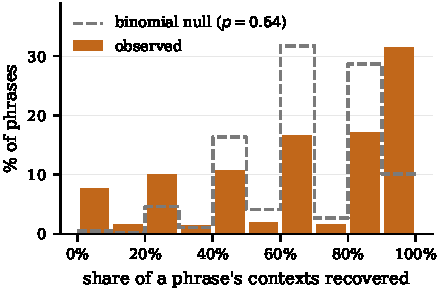
\includegraphics[width=\columnwidth]{figures/per_phrase_consistency}
\caption{Share of its own distinct contexts in which each phrase's continuation
is recovered at $i=3$, generation readout, over the $803$ phrases with at least
five distinct contexts. The dashed line is the binomial distribution expected if
every context were an independent draw at the pooled rate $p=0.64$. The observed
distribution puts mass at both extremes, where the null has almost none.}
\label{fig:consistency}
\end{figure}

An aggregate rate of $64.8\%$ at $i=3$ is consistent with two very different
pictures. Either the model recovers most phrases most of the time with some
per-occasion noise, or it reliably recovers some phrases and reliably fails on
others. Only the second supports the idea of a stable, reusable phrase-level
representation.

For each of the $803$ phrases with at least five distinct contexts
(\S\ref{sec:setup}) we compute the share of its contexts that succeed, and
compare the resulting distribution against the binomial null in which every
context is an independent draw at the pooled rate $p = 0.645$
(Figure~\ref{fig:consistency}). The two differ sharply. $31.5\%$ of phrases
succeed in at least $90\%$ of their contexts where the null predicts $10.1\%$,
and $18.3\%$ succeed in at most $20\%$ where the null predicts $5.0\%$;
conversely only $27.3\%$ fall in the $40$--$60\%$ band that holds $48.5\%$ of
the null's mass. The Patchscopes readout is more extreme still, at $37.4\%$ and
$22.5\%$ against nulls of $9.5\%$ and $5.4\%$.

We read this as evidence that what varies is the phrase, not the occasion. Some
expressions are reliably available to the model ahead of time and others are
reliably not, and context modulates that availability rather than creating it.
This is what makes the probing question in \S\ref{sec:probe} worth asking: a
signal that is stable per phrase is a signal that something in the
representation could carry.

\subsection{Where in the model the phrase becomes readable}
\label{sec:layers}

\begin{figure}[t]
\centering
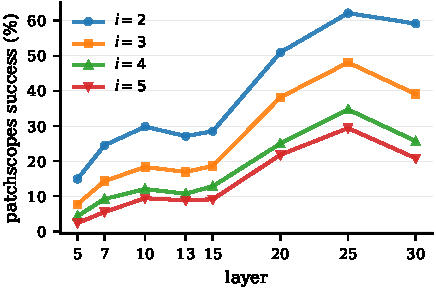
\includegraphics[width=\columnwidth]{figures/patchscopes_by_layer}
\caption{Patchscopes success by layer and lookahead distance, in context, over
the eight probed layers. Recovery rises through the network, peaks at L25, and
falls at L30 at every distance.}
\label{fig:bylayer}
\end{figure}

Recording Patchscopes success separately at each of the eight probed layers
(Figure~\ref{fig:bylayer}) gives a consistent shape across all four distances:
recovery is low in the early layers, rises through the middle of the network,
peaks at L25 --- $62.2\%$ at $i=2$, $48.1\%$ at $i=3$ --- and then falls back at
L30, to $59.2\%$ and $39.1\%$. The decline in the last layers appears at every
$i$ and in every category.

One explanation is that the final layers specialise toward producing the actual
next token for the real input rather than maintaining a general, transferable
representation, so a state lifted from L30 and pasted into an unrelated prompt
transfers less well than one lifted from L25. We note that this is a hypothesis
consistent with our data and with the late-layer decline reported by
\citet{kaplan-etal-2025-tokens} for word-level retrieval, not something these
experiments establish; a state that a patchscope can no longer verbalise may
still carry the information in a form the rest of the network can use.

Taking the union over all $32$ layers rather than eight, the median first
successful layer is L16, and $41.9\%$ of successes first appear at or before
L10 (Appendix~\ref{app:details}). Phrase information thus becomes readable
gradually and, for a large minority of cases, quite early.

\subsection{The two readouts disagree}
\label{sec:disagreement}

\begin{table}[t]
\centering\small
\begin{tabular}{rrrrrrr}
\toprule
$i$ & $n$ & both & \makecell{ps.\\only} & \makecell{gen.\\only} & neither & \makecell{agree\\(\%)} \\
\midrule
2 & 9,148 & 6,757 & 521 & 923 & 947 & 84.2 \\
3 & 8,529 & 4,681 & 783 & 849 & 2,216 & 80.9 \\
4 & 4,677 & 1,968 & 445 & 632 & 1,632 & 77.0 \\
5 & 2,386 & 933 & 175 & 347 & 931 & 78.1 \\
\midrule
2--5 & 24,740 & 14,339 & 1,924 & 2,751 & 5,726 & 81.1 \\
\bottomrule
\end{tabular}
\caption{Patchscopes (32-layer union) and generation on \emph{identical}
(phrase, context, $i$) instances. The two readouts disagree on
18.9\% of instances, and the disagreement runs in both
directions: 1,924 instances are recovered only by
patchscopes and 2,751 only by generation.}
\label{tab:agreement}
\end{table}

\begin{table}[t]
\centering\small
\begin{tabular}{lrrr}
\toprule
& & \multicolumn{2}{c}{\textbf{Recovery (\%)}} \\
\cmidrule(lr){3-4}
\textbf{Category} & \textbf{Inst.} & patchscopes & generation \\
\midrule
Landmarks & 1,409 & 56.8 & 75.3 \\
Idioms & 20,371 & 65.9 & 66.4 \\
Film titles & 2,960 & 68.6 & 84.5 \\
\bottomrule
\end{tabular}
\caption{Recovery by phrase category, pooled over $i=2\ldots5$, in natural
context. The two readouts order the categories differently: under generation,
idioms are the hardest category, while under patchscopes they sit between
landmarks and film titles.}
\label{tab:categories}
\end{table}


So far we have reported both readouts as if they were interchangeable
measurements of one underlying quantity. They are not. Table~\ref{tab:agreement}
compares them on identical instances --- same phrase, same context, same cut
point, same success criterion --- and they agree on $78.7\%$ of the $24{,}740$
pooled trials.

The residual $21.3\%$ is the informative part. It is lopsided: generation
recovers a continuation that Patchscopes misses in $15.7\%$ of instances, while
Patchscopes recovers one that generation misses in only $5.6\%$ --- roughly a
three-to-one asymmetry. Read on its own, that says Patchscopes undercounts what
the model can do.

But the two failure directions are qualitatively different, and neither is
simply an instrument defect. Where Patchscopes succeeds and generation does not,
the state does contain the phrase --- the patchscope verbalises it --- yet the
real context steers the model elsewhere; given \textit{Why should one person be
brought up}, the model writes \textit{a wealthy family, with every opportunity}
instead of completing \textit{in the lap of luxury}. Where generation succeeds
and Patchscopes does not, the model completes the phrase correctly from its real
prefix while the patchscope, at the same position, reaches for a neighbouring
expression: for \textit{a bird in the hand is worth two in the bush} it returns
\textit{worth more than one}. The first is a continuation that was available but
not taken; the second is a readout that recovered the sense and lost the
wording.

\paragraph{The asymmetry is partly a layer-budget artifact.}
The comparison above gives Patchscopes eight layers. Sweeping all $32$ raises
its in-context rate from $73.2\%$ to $79.6\%$ at $i=2$ and from $38.7\%$ to
$46.4\%$ at $i=5$ (Table~\ref{tab:main}), lifts agreement to $81.1\%$, and
rebalances the disagreement from three-to-one to roughly three-to-two
(Table~\ref{tab:agreement}). At $i=3$ the two readouts then differ by $0.7$
points overall. Most of the apparent superiority of generation is therefore a
statement about how thoroughly Patchscopes was sampled, not about the model.
What survives the wider sweep is the disagreement itself: even at $32$ layers,
$18.9\%$ of instances are classified differently, and $7.8\%$ are recovered only
by Patchscopes. The two instruments are not nested, and no layer budget makes
one a refinement of the other.

We use the eight-layer readout as our primary measurement because it is the
layer set on which every per-layer, per-category and probing analysis in this
paper was run, so all of those results are mutually consistent. Readers
comparing our Patchscopes rates against other work should note that the budget
moves them by six to eight points.

\paragraph{Category difficulty is readout-dependent.}
Table~\ref{tab:categories} breaks the pooled rates down by phrase kind, and the
two readouts do not merely differ in level --- they reverse an ordering. Under
Patchscopes, idioms are the \emph{easiest} category at $57.4\%$, ahead of film
titles ($54.7\%$) and landmarks ($47.2\%$). Under generation, idioms are the
\emph{hardest} at $66.4\%$, well behind film titles ($84.5\%$) and landmarks
($75.3\%$). The reversal is consistent with the scoring artifact of
\S\ref{sec:falsepos}: idioms have accepted variants, so exact-match scoring
penalises them most under the readout that produces the most fluent
continuations. Under the wider $32$-layer sweep idioms move to the middle of the
Patchscopes ranking rather than the top, so the reversal weakens to a
re-ordering, but the categories are still ranked differently by the two
instruments.

The practical consequence is narrow but real. A study measuring only with
Patchscopes would report that this model handles idioms better than landmarks or
titles; one measuring only with generation would report the opposite. Both would
be reporting their instrument as much as their model.

\subsection{The hidden state predicts real completion}
\label{sec:probe}

\begin{table}[t]
\centering\small
\begin{tabular}{rrrrrr}
\toprule
& \multicolumn{3}{c}{\textbf{Patchscopes label}} & \multicolumn{2}{c}{\textbf{Generation label}} \\
\cmidrule(lr){2-4}\cmidrule(lr){5-6}
\textbf{Layer} & pos.\ (\%) & bal.\ acc. & prec. & bal.\ acc. & prec. \\
\midrule
5 & 6.6 & 76.0 & 33.9 & 69.8 & 83.3 \\
7 & 14.7 & 70.2 & 42.8 & 71.0 & 84.2 \\
10 & 18.8 & 76.5 & 52.3 & 72.0 & 84.9 \\
13 & 16.9 & 74.8 & 45.8 & 73.6 & 85.6 \\
15 & 18.5 & 76.3 & 51.1 & 74.2 & 86.1 \\
20 & 36.8 & 70.4 & 62.4 & 73.6 & 85.8 \\
25 & 47.7 & 68.1 & 67.2 & 74.6 & 86.2 \\
30 & 40.2 & 66.4 & 59.7 & 76.8 & 87.6 \\
\bottomrule
\end{tabular}
\caption{Probes trained on the hidden state at the cut position to predict each
readout's outcome, pooled over $i=2\ldots5$, split by phrase (80/20), training
set class-balanced by downsampling, evaluated on the natural test distribution.
The generation label has a fixed positive rate of 69.1\% at every
layer; the patchscopes label does not, which is why its raw accuracy is not
comparable across layers. Balanced accuracy for the patchscopes label peaks in
the middle of the model, whereas for the generation label it rises
monotonically with depth.}
\label{tab:probes}
\end{table}


\begin{figure}[t]
\centering
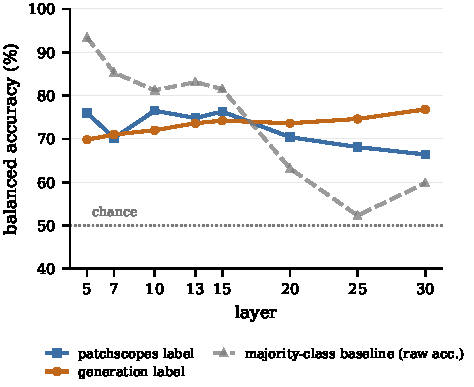
\includegraphics[width=\columnwidth]{figures/probe_balanced_accuracy}
\caption{Balanced accuracy of the two probes by layer. The label determines the
shape: predicting Patchscopes success peaks in the middle layers, while
predicting real completion rises monotonically to L30.}
\label{fig:probes}
\end{figure}

If phrase anticipation is carried by the representation, it should be readable
from the representation without an intervention. We train a small MLP
($32$ hidden units) on the raw hidden state at the cut position to predict, as a
binary label, whether the readout succeeds. Data are pooled over
$i \in \{2,3,4,5\}$ and split by phrase at $80/20$, so no test phrase appears in
training; the training set is class-balanced by downsampling and the test set is
left at its natural distribution.

Predicting \emph{real completion} works well. Balanced accuracy rises
monotonically with depth, from $69.8\%$ at L5 to $76.8\%$ at L30, and precision
is high and nearly flat at $83.3\%$ to $87.6\%$ (Table~\ref{tab:probes}). A
positive call from this probe is right roughly seven times in eight, and it is
made from a single hidden vector, before the model has produced any of the
tokens in question.

\paragraph{The signal is learned, not a base rate.}
Because $69.1\%$ of instances are positive, a probe could score respectably by
guessing. Two checks argue against that reading. First, balanced accuracy
corrects for the base rate by construction, and the probe clears $50\%$
everywhere. Second, running the same probe on the earliest layers gives a clean
gradient: $58.6\%$ balanced accuracy at L0 --- the raw embedding, before any
contextual processing --- rising to $65.1\%$ at L1, $66.5\%$ at L2 and $69.8\%$
at L5. A base-rate artifact would be flat across layers; this climbs as
computation accumulates. We note nonetheless that $58.6\%$ at L0 is above
chance, which suggests some of the signal is carried by lexical identity of the
cut token rather than by contextual processing.

\paragraph{The label changes where the ``best'' layer is.}
Training the identical architecture on the Patchscopes label instead produces a
different profile: balanced accuracy peaks in the middle of the network
($76.5\%$ at L10, $76.3\%$ at L15) and is worst at L30 ($66.4\%$), the mirror
image of the generation-label curve (Figure~\ref{fig:probes}). Raw accuracy for
this probe is not comparable across layers at all, because the positive rate
moves from $6.6\%$ at L5 to $47.7\%$ at L25 as Patchscopes itself gets better.
A reader interested in \emph{where in the model phrase information lives} would
draw opposite conclusions from the two probes. We read the generation-label
probe as the more trustworthy of the two, since its label does not depend on the
layer being probed, but the divergence is itself the point.

\subsection{Most apparent errors are valid alternates}
\label{sec:falsepos}

The probe's precision is bounded by the scoring criterion, not only by the
model. We adjudicated all $412$ false positives of the generation-label probe at
L25 --- cases where the probe predicted completion and exact-match scoring
recorded a failure --- using an LLM judge asked whether the generated text means
the same as the target. It labelled $62.9\%$ valid alternates,
$17.5\%$ partially correct and $19.7\%$ unrelated. Typical valid alternates are
\textit{laughs best} for \textit{laughs loudest}, \textit{plowshares} for
\textit{ploughshares}, and \textit{beat around the bush} for \textit{beat about
the bush}: the more common form of the expression, scored as a failure.

Read cautiously --- this is a single unvalidated judge, and we report it as
indicative rather than as a corrected accuracy --- it suggests that roughly four
in five of these apparent errors reflect the rigidity of exact matching rather
than a model that did not know the phrase. The direction of the bias is
consistent across our analyses: our reported rates are conservative.

\paragraph{The model's own confidence tracks the real outcome.}
Averaging the probability the model assigns to each token it generates, mean
confidence is $0.878$ on successful completions and $0.447$ on failures. Split
by probe outcome at L25, confidence follows the true label rather than the
probe's guess: true positives average $0.904$ and false negatives $0.791$, while
false positives average $0.599$ and true negatives $0.414$. Where the probe is
wrong, the model was not.

\section*{Limitations}
\label{sec:limitations}

\paragraph{Scoring is at the token level, not the word level.}
The target is the decoded string of the final $i$ tokens, which for some phrases
begins mid-word: at $i=2$ in \textit{Sistine Chapel} the target is
\textit{istine Chapel}, and in \textit{Pulp Fiction} it is \textit{ulp Fiction}.
The criterion is applied identically to both readouts, so comparisons between
them are unaffected, but absolute rates for phrases with unusual tokenization
are not directly interpretable as ``the model produced the phrase''. Rerunning
with word-aligned cut points would make the absolute numbers cleaner.

\paragraph{Exact matching both over- and under-counts.}
Substring containment credits any output that includes the target, without
requiring that the model produced it for the right reason, and penalises
accepted variants of the same expression (\S\ref{sec:falsepos}). The
adjudication in \S\ref{sec:falsepos} suggests the net bias is conservative, but
it rests on a single judge with no human validation and no inter-annotator
agreement, and the specific ChatGPT model version used was not recorded at the
time, so that run is not exactly reproducible. The prompt is in
Appendix~\ref{app:judge} and the analysis should be rerun with a named model
before the number is relied on. The confidence-based split in
\S\ref{sec:falsepos}, which uses no judge, is the more reproducible of the two
and points the same way.

\paragraph{One model family carries most of the weight.}
All layer-level and probing results are from OLMo-2-7B. We replicate the
lookahead curves on OLMo-3-7B and the generation readout on Qwen2.5-14B
(Appendix~\ref{app:details}), and the qualitative pattern holds, but we have not
established that the layer localisation or the probe's profile transfers. The
Qwen2.5-14B result is worth flagging in its own right: at roughly twice the
parameters it does not clearly outperform OLMo-2-7B on this task, which suggests
that phrase anticipation is not simply a function of general model capability.

\paragraph{Contexts are duplicated in the collected set.}
Of the $9{,}955$ (phrase, context) instances, $44.8\%$ are repeats of a context
already present for the same phrase, an artifact of how the collection was
resumed (\S\ref{sec:setup}). Aggregate rates barely move under deduplication and
per-phrase analyses are computed over distinct contexts only, but the effective
sample size behind every instance-level number is closer to $5{,}498$ than to
$9{,}955$. Any confidence interval computed from the instance count would be too
narrow, which is one reason we report no significance tests. The per-layer and
probing analyses were run over the duplicated set and were not recomputed.

\paragraph{The phrase set is narrow and English-only.}
We deliberately chose frequent, fixed English expressions as a favourable case.
Nothing here speaks to compositional continuations, to rarer expressions, or to
other languages, and the three categories are unbalanced: idioms are $82\%$ of
pooled instances, so aggregate rates are close to idiom rates.

\paragraph{The Patchscopes readout is sampled, not exhaustive.}
Our primary measurement unions eight of the model's $32$ layers, chosen so that
every per-layer, per-category and probing result rests on the same states. That
undercounts what a full sweep recovers by six to eight points, and it is the
single largest contributor to the apparent asymmetry between the two readouts
(\S\ref{sec:disagreement}). We report the $32$-layer sweep wherever we have it,
but it is not available for the per-category or probing analyses, so those
should be read as lower bounds on Patchscopes performance. A budget-matched
comparison across every analysis would require storing hidden states for all
$32$ layers at every trial.

\paragraph{Probe results are not reproducible from the released artifacts.}
The probing experiments require per-trial hidden states --- $1.28$\,GB for the
Patchscopes labels and $3.02$\,GB for the generation labels --- which are too
large to distribute and remain on the compute cluster. They are intact, so the
runs can be reproduced there, but the probe numbers in Table~\ref{tab:probes}
are reported from the run logs rather than recomputed from this repository's
result files, unlike every other number in the paper.

\paragraph{No efficiency claim is tested.}
The motivation in \S\ref{sec:intro} is that anticipation could be exploited to
skip computation, and the probe's precision is high enough to make that worth
investigating. We did not implement any such decoding scheme and report no
latency or throughput measurement. Whether a probe of this kind is cheap enough
to pay for itself is an open question.

\section*{Ethics Statement}

This work analyses publicly available language models on publicly available
text. The phrase sets are drawn from published idiom corpora and public lists of
landmarks and film titles; the contexts are sampled from FineWeb-Edu, a filtered
web corpus whose documents we did not inspect individually and which may contain
the biases of web text. We do not release any model, and the analysis does not
involve human subjects or personal data. The efficiency direction this work
motivates, if pursued, would reduce inference cost; we make no claim to have
demonstrated that reduction here.

\section{Conclusion}
\label{sec:conclusion}

We asked whether a language model's internal state, partway through a familiar
multi-word expression, already encodes the rest. For fixed expressions in
natural text the answer is yes, and at a useful range: OLMo-2-7B completes such
phrases three tokens early in roughly two thirds of instances and five tokens
early in more than half. The ability is a stable property of the phrase rather
than of the occasion: across a phrase's natural contexts, success clusters at
the extremes far more than independent per-context variation would produce. It
is also legible from the representation itself, well enough that a small probe reading a single hidden
vector predicts real completion at $87.6\%$ precision.

The second finding is a caution about how the first was obtained. Patchscopes
and ordinary generation, run on identical instances, agree on only $78.7\%$ of
them, reverse the ranking of the phrase categories, and, used as probe labels,
locate the relevant information in different parts of the network. Part of that
gap is a budget we chose, since widening the sweep from eight layers to all $32$
recovers six to eight points, but the disagreement itself survives the widest
sweep we can run. Neither instrument is wrong; neither is a neutral window onto
what the model knows. Claims of the form \emph{the model already knows $X$}
should carry the readout that produced them, and the budget it was given.

The practical thread we have not pulled is efficiency. A signal that is stable
per phrase, available from mid-network states, and precise enough to act on is
the kind of signal a decoding scheme could use to commit several tokens at once
rather than paying full depth for each. We are pursuing that direction
separately, as an adaptive multi-token prediction policy checked token by token
against an autoregressive baseline; nothing in the present paper depends on its
outcome. An early pilot there is instructive about the size of
the prize: reproducing CLP \citep{xie-zhou-2026-clp}, a learned linear read of
the hidden state that sets the draft length per step, on a different model, we
measured roughly $1.34\times$ the throughput of plain autoregressive decoding.
A policy that simply drafts a fixed number of tokens at every step was faster
still, at $1.72\times$, while diverging from the autoregressive output
more often.\footnote{Three caveats on that pilot. Our figure exceeds the
$1.14\times$--$1.29\times$ Xie and Zhou report, which we take to reflect
differences in model, hardware and workload rather than a stronger
implementation. We observed occasional divergences from autoregressive output
under \emph{every} drafting policy we tried, including fixed-length ones with no
adaptive logic at all, which points at this model's interaction with the
inference engine rather than at any policy. And those divergences were more
common for the more aggressive fixed-length policies (six of ten prompts,
against two for CLP), so the fixed-length speed advantage is not free.}
Ten held-out prompts settle nothing either way. What the pilot does suggest is
that the open question is not whether anticipation exists, which this paper settles,
but whether reading it out adaptively buys enough over drafting blindly to pay
for itself.


\bibliography{anthology-1,anthology-2,custom}

\appendix
\section{Experimental Details and Supporting Analyses}
\label{app:details}

\subsection{Implementation}

Hidden states are extracted with a single forward pass over
\texttt{[BOS]} $+$ context $+$ phrase, with \texttt{output\_hidden\_states}
enabled. The BOS token is required: the state of a phrase's first token at
position $0$ differs substantially from its state at position $1$ after a BOS,
and omitting it produces degenerate patchscope outputs.\footnote{This was the
source of a long-lived bug in an earlier version of this work, in which
patchscope outputs for well-known phrases were unrelated to the input.}
Positions are enumerated from the first phrase token to the second-to-last; the
BOS and the final phrase token are never cut points.

For the Patchscopes readout, the states for all probed layers are stacked into
one batch and decoded in a single \texttt{generate} call, so the layer sweep
costs one generation pass rather than one per layer. Decoding is greedy
throughout, for both readouts, with \texttt{max\_new\_tokens} $= i+3$.

\subsection{Patchscope prompt ablation}

The prompt \texttt{"Repeat this: X"} offers one slot for the injected state.
Because the target is several tokens long, a natural worry is that one slot is
too little room. We reran the isolated-phrase sweep with
\texttt{"Repeat this: X X X X X"}, injecting the same state into five slots.
It does not help, and at longer distances it hurts: $27.4\%$ versus $30.9\%$ at
$i=3$, $15.8\%$ versus $19.4\%$ at $i=4$, and $12.4\%$ versus $16.5\%$ at
$i=5$. We therefore use the single-slot prompt throughout. The failure mode at
long $i$ is not a shortage of output positions.

\subsection{Replication across models}

\begin{table}[t]
\centering\small
\begin{tabular}{llrrrr}
\toprule
& & \multicolumn{4}{c}{$i$} \\
\cmidrule(lr){3-6}
\textbf{Model} & \textbf{Readout} & 2 & 3 & 4 & 5 \\
\midrule
\multicolumn{6}{l}{\textit{Phrase in isolation}} \\
OLMo-2-7B & patchscopes & 57.8 & 30.9 & 19.4 & 16.5 \\
OLMo-3-7B & patchscopes & 40.4 & 20.1 & 11.8 & 9.9 \\
OLMo-2-7B & generation & 59.2 & 31.2 & 20.6 & 17.6 \\
Qwen2.5-14B & generation & 54.3 & 28.4 & 18.8 & 17.4 \\
\midrule
\multicolumn{6}{l}{\textit{Phrase in natural context}} \\
OLMo-2-7B & patchscopes & 79.6 & 64.1 & 51.6 & 46.4 \\
OLMo-3-7B & patchscopes & 71.4 & 52.8 & 38.9 & 32.9 \\
OLMo-2-7B & generation & 84.0 & 64.8 & 55.6 & 53.6 \\
Qwen2.5-14B & generation & 84.8 & 66.2 & 57.4 & 54.7 \\
\bottomrule
\end{tabular}
\caption{Recovery rate (\%) across models, on the same phrase strings and
contexts. Each model uses its own tokenizer, so $i$ counts model-specific tokens
and the cut points need not coincide across rows. Patchscopes rows are the union
over all 32 layers. Qwen2.5-14B, at
roughly twice the parameters of OLMo-2-7B, is slightly behind it in isolation
and slightly ahead of it in context.}
\label{tab:replication}
\end{table}


Table~\ref{tab:replication} repeats the central measurement on OLMo-3-7B
(both readouts share the OLMo-2 protocol; note that this tokenizer does not
prepend a BOS token) and on Qwen2.5-14B (generation readout only). The
qualitative picture is stable across all three: anticipation several tokens
ahead, a large context effect, and a monotone decline with $i$. The absolute
levels differ, and not in the direction model scale would predict --- OLMo-3-7B
is consistently below OLMo-2-7B, and Qwen2.5-14B, at roughly twice the
parameters, trails OLMo-2-7B in isolation and leads it by one to two points in
context.

\subsection{Depth of first recovery}

\begin{figure}[t]
\centering
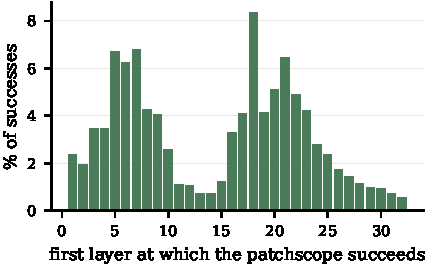
\includegraphics[width=\columnwidth]{figures/first_successful_layer}
\caption{Over the full $32$-layer sweep with context, the first layer at which
the patchscope recovers the target, as a fraction of all successes.}
\label{fig:firstlayer}
\end{figure}

Figure~\ref{fig:firstlayer} shows, across the $26{,}015$ successful in-context
trials of the $32$-layer sweep, which layer first produced the target. The
distribution has two modes, one around L5--L8 and a larger one around L18--L22;
the median is L16 and $41.9\%$ of successes first appear at or before L10. The
early mode is not visible in the eight-layer analysis of \S\ref{sec:layers},
which samples only L5 and L7 below L10.

\subsection{Probe generalisation to unseen categories}

Training the generation-label probe on two phrase categories and testing on the
third costs accuracy but does not eliminate the signal. Against a no-hold-out
baseline of $73.6\%$ / $74.6\%$ / $76.8\%$ balanced accuracy at L13 / L25 / L30,
holding out landmarks gives $69.1\%$ / $62.6\%$ / $63.4\%$, idioms
$68.7\%$ / $68.9\%$ / $72.3\%$, and film titles
$72.4\%$ / $72.7\%$ / $73.5\%$. Landmarks are the hardest category to
generalise to, which is unsurprising given that they are only $5.7\%$ of pooled
instances. The probe is therefore learning something that partly transfers
across phrase types rather than memorising category-specific surface features,
but the transfer is imperfect --- a pattern also reported by
\citet{orgad-etal-2025-llms} for truthfulness probes across datasets.

\subsection{Per-phrase correlation between probe confidence and difficulty}

A complementary check on whether the probe tracks phrase identity: for each test
phrase, we compare the probe's mean predicted probability across that phrase's
contexts with the phrase's true success rate. At $i=3$ over $180$ test phrases,
Pearson correlation by layer is $0.413$ (L5), $0.551$ (L7), $0.621$ (L10),
$0.584$ (L13), $0.603$ (L15), $0.556$ (L20), $0.517$ (L25) and $0.480$ (L30) ---
a broad mid-network peak. The probe's confidence therefore varies with which
phrase it is looking at, not only with generic features of the position.

\subsection{Reproducing the numbers}

Every number in the main text except Table~\ref{tab:probes} and the
adjudication of \S\ref{sec:falsepos} is recomputed from the files in
\texttt{results/raw/} by \texttt{code/make\_paper\_numbers.py}, which writes
\texttt{results/processed/paper\_numbers.json}; the tables and figures are
generated from that file by \texttt{code/make\_tables.py} and
\texttt{code/make\_figures.py}. The experiment scripts are in
\texttt{code/phrase\_recognition/}. Per-trial hidden states, which the probing
experiments require, are not distributed.


\end{document}
